\chapter{Validierung}\label{chap4}

Für jede Simulation ist von großer Bedeutung, wie weit Ergebnisse mit der Realität übereinstimmen, deshalb möchten wir dies im folgenden Abschnitt näher untersuchen. Dabei wollen wir auf zwei mögliche Fehlerursachen eingehen, zum einen die Richtigkeit der Modellierung und zum anderen die Umsetzung der Implementierung. 
\\ \\
Um unsere Implementierung zu prüfen, haben wir mehrere Faktoren betrachtet. Viele Fehler kann man bereits bei der Betrachtung der Animation sehen, bewegen sich die Autos wie erwartet, oder gibt es Unregelmäßigkeiten? So konnten viele Fehler während der Entwicklungsphase entdeckt und anschließend ausgeräumt werden. Natürlich gibt es auch Fehler, die nicht so einfach gefunden werden können, daher haben wir einige Tests durchgeführt. Unter anderem haben wir geprüft, ob die Anzahl der Autos während einer Simulation konstant bleibt, dass also keine Autos verschwinden oder plötzlich auftauchen. Auch haben wir dank der Mitspeicherung der Autonummer sehen können, dass die Reihenfolge immer gleich bleibt. 
\\ \\ 
Ein wichtiges Tool für die Validierung ist das Fundamentaldiagramm, es stellt den Zusammenhang zwischen der Dichte und dem Verkehrsfluss dar. Da bei unserer Kreuzung der Fluss hauptsächlich von der Dichte auf der vertikalen Ringstraße abhängt, ist bei unseren Diagrammen immer die vertikale Dichte auf der $x$-Achse angetragen. 
\\ \\
Um das Fundamentaldiagramm zu erstellen, muss man den Verkehrsfluss $f$ und die Verkehrsdichte $\rho$ bestimmen. Der Verkehrsfluss $f$ an einem bestimmten Messpunkt ist bestimmt durch
\[ f = \frac{P}{\delta T}. \]
Wobei $P$ die Anzahl der Autos ist, die den Messpunkt während des Zeitintervalls $\delta T$ passiert haben. In unserem Fall haben wir dieses Intervall $\delta T$ auf die gesamte Simulationsdauer (ungefähr $100$ Sekunden) festgelegt. Als Messpunkt haben wir uns auf die Kreuzung festgelegt, da diese Stelle am interessantesten ist, im Programm kann man den Messpunkt aber auch verschieben. Für die Dichte haben wir die gesamte Dichte auf der vertikalen Ringstraße verwendet, dies kann durch folgende Formel
\[ \rho = \frac{N}{L} \]
bestimmt werden. $N$ ist hierbei die Anzahl der Autos auf der vertikalen Straße und $L$ ist die totale Länge der Ringstraße. Diese Vorgehensweise ist auch in \cite{book:bungartz} Abschnitt 8.3.3 zu finden, allerdings haben wir einen Spezialfall davon verwendet, da bei uns die Variable $L$ gleich der gesamten Straßenlänge ist.

\begin{figure}[H]%
\centering
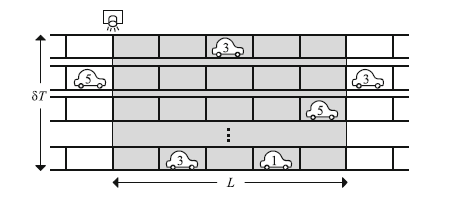
\includegraphics[width=8cm]{4_BestFD.png}%
\caption[Messung von Fluss und Dichte in der Simulation]{Bestimmung des Verkehrsflusses und der Verkehrsdichte, in unserem Fall ist $\delta T$ gleich den gesamten Simulationsschritte und $L$ ist die gesamte Straßenlänge. Quelle: \cite{book:bungartz} Abb. 8.8}%
\label{pic:FD_Skizze}%
\end{figure}
\noindent
Zunächst konnten wir unsere Ergebnisse mit den Resultaten aus \cite{book:bungartz} für eine einfache Ringstraße vergleichen. Dafür haben wir die Kreuzungsdaten aus unserem Tool entfernt, dadurch simulieren wir eine einfache Ringstraße ohne Hindernisse. In der Abbildung \ref{pic:FD_Vergleich} werden die unterschiedlichen Diagramme dargestellt. Aufgrund der hohen Ähnlichkeit können wir grobe Implementierungsfehler im Grundgerüst unseres Programmes ausschließen.

\begin{figure}[H]%
\centering
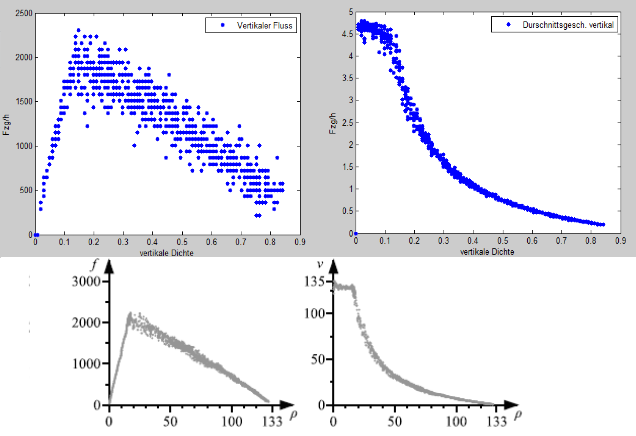
\includegraphics[width=12cm]{4_FD_Vergleich.png}%
\caption[Fundamentaldiagramm]{Oben: Unsere erzeugten Diagramme Unten: Diagramme aus \cite{book:bungartz} Abb. 8.9. Jeweils mit Trödelwahrscheinlichkeit $p=0.2$}%
\label{pic:FD_Vergleich}%
\end{figure} 
\noindent
Ein weiteres visuelles Tool zur Darstellung unserer Simulation sind die Zellen-Zeit-Diagrammen. Hierbei wird für jedes Auto zu jedem Zeitschritt die Position in einem Koordinatensystem dargestellt. Zwei solche Diagramme sind in in Abbildung \ref{pic:ZelleZeit} dargestellt. Somit kann mithilfe eines Bildes die gesamte Simulation visualisiert werden. Dadurch können auch Fehler sofort entdeckt werden und die Simulation auf ihre Richtigkeit überprüft werden. 
\begin{figure}[H]%
\centering
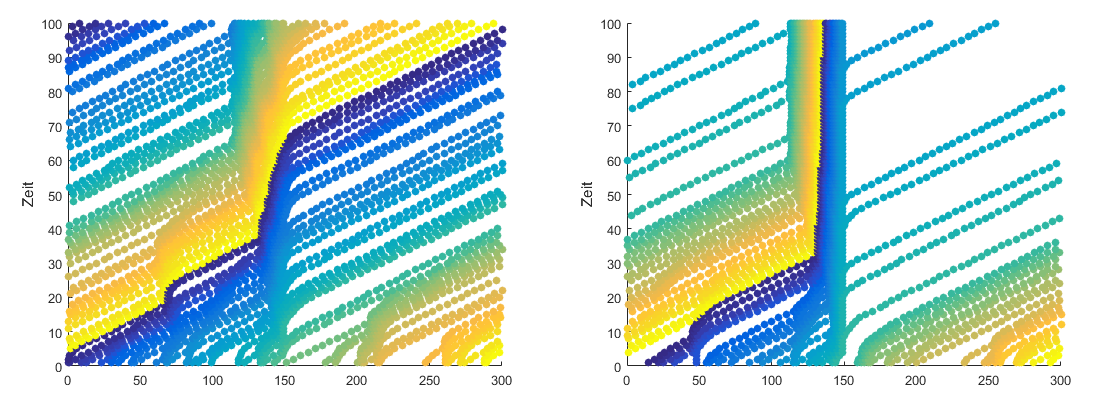
\includegraphics[width=15cm]{4_ZelleZeit.png}%
\caption[Zellen-Zeit-Diagramm]{Links: Das Zellen-Zeit-Diagramm für die vertikale Ringstraße mit Dichte $\rho_v = 0.11$. Rechts: Analog die dazugehörige horizontale Straße mit Dichte $\rho_h=0.12$. Gemeinsame Trödeldichte ist $0.2$ und die gesamte Straßenlänge beider Ringstraßen ist $300$ Zellen, die Kreuzung befindet sich an der Stelle 150.  }%
\label{pic:ZelleZeit}%
\end{figure}
\noindent
In unseren Zellen-Zeit-Diagrammen besitzt jedes Auto eine eigene Farbe, so kann man schnell die Trajektorie eines Fahrzeugs ablesen. Auch würden so unnatürliches Verhalten der Autos sofort erkannt werden. Schön zu sehen ist das Verhalten der Autos nahe der Kreuzung. Bei der vertikalen Straße bremsen die Autos kurz vor der Kreuzung ab, fahren aber dann relativ zügig über die Kreuzung. Dagegen wird bei der horizontalen Straße meist schon früher abgebremst, da sich ein Rückstau aufgrund der Rechts vor Links Regel ergibt. So kann es passieren, dass Autos über viele Zeitschritte auf eine Weiterfahrt warten müssen. Diese Wartezeit ist, wie auch zu erwarten, von der Dichte der vertikalen Straße abhängig. Somit verhalten sich die Ergebnisse unsere Simulation genauso, wie man vermutet hätte.

\begin{flushright}
Autor: Martin Kraus
\end{flushright}